% MIT License
%
% Copyright (c) 2021 Geoffrey H. Garrett
%
% Permission is hereby granted, free of charge, to any person obtaining a copy
% of this software and associated documentation files (the "Software"), to deal
% in the Software without restriction, including without limitation the rights
% to use, copy, modify, merge, publish, distribute, sublicense, and/or sell
% copies of the Software, and to permit persons to whom the Software is
% furnished to do so, subject to the following conditions:
%
% The above copyright notice and this permission notice shall be included in all
% copies or substantial portions of the Software.
%
% THE SOFTWARE IS PROVIDED "AS IS", WITHOUT WARRANTY OF ANY KIND, EXPRESS OR
% IMPLIED, INCLUDING BUT NOT LIMITED TO THE WARRANTIES OF MERCHANTABILITY,
% FITNESS FOR A PARTICULAR PURPOSE AND NONINFRINGEMENT. IN NO EVENT SHALL THE
% AUTHORS OR COPYRIGHT HOLDERS BE LIABLE FOR ANY CLAIM, DAMAGES OR OTHER
% LIABILITY, WHETHER IN AN ACTION OF CONTRACT, TORT OR OTHERWISE, ARISING FROM,
% OUT OF OR IN CONNECTION WITH THE SOFTWARE OR THE USE OR OTHER DEALINGS IN THE
% SOFTWARE.

%%%%%%%%%%%%%%%%%%%%%%%%%%%%%%%%%%%%%%%%%%%%%%%%%%%%%%%%%%%%%%%%%%%%%%%%%%%%%%%
% ACKNOWLEDGEMENTS
%%%%%%%%%%%%%%%%%%%%%%%%%%%%%%%%%%%%%%%%%%%%%%%%%%%%%%%%%%%%%%%%%%%%%%%%%%%%%%%
% Design and implementation of this diagram was inspired and adapted from:
% https://tex.stackexchange.com/questions/573127/tikz-plots-are-not-centered

%%%%%%%%%%%%%%%%%%%%%%%%%%%%%%%%%%%%%%%%%%%%%%%%%%%%%%%%%%%%%%%%%%%%%%%%%%%%%%%
% DEPENDENCIES
%%%%%%%%%%%%%%%%%%%%%%%%%%%%%%%%%%%%%%%%%%%%%%%%%%%%%%%%%%%%%%%%%%%%%%%%%%%%%%%
%\usepackage{tikz}
%\usepackage{amsmath}

%%%%%%%%%%%%%%%%%%%%%%%%%%%%%%%%%%%%%%%%%%%%%%%%%%%%%%%%%%%%%%%%%%%%%%%%%%%%%%%
% USER STYLING
%%%%%%%%%%%%%%%%%%%%%%%%%%%%%%%%%%%%%%%%%%%%%%%%%%%%%%%%%%%%%%%%%%%%%%%%%%%%%%%

%\begin{tikzpicture}
%    \begin{axis}[
%        xmin=-4,
%        xmax=4.5,
%        ymin=-0.5,
%        ymax=3.5,
%        ticks=none,
%        xticklabels={\empty},
%        yticklabels={\empty},
%        ymajorgrids=false,
%        xmajorgrids=false,
%        axis line style = semithick,
%        axis equal image,
%%        width=1.2\columnwidth
%    ]
%    \draw (axis cs:0,3) circle [blue, radius=1];
%    \end{axis}
%\end{tikzpicture}


\newcommand{\plotregularizercontour}[2] {
%        \addplot[dashed, dash phase=0.1em, thick, color=#2, draw opacity=1, mark=none, fill=#2, fill opacity=0.01] coordinates {
%            (#1, 0)
%            (0, -#1)
%            (-#1, 0)
%            (0, #1)
%            (#1, 0)
%        };
    \draw[dashed, dash phase=0.1em, fill=cyan!20, fill opacity=0.4] (axis cs:0,0) circle [#2, radius=#1];

}

\newcommand{\plotobjectivecontour}[6] {
    \draw[#6, thin] (#1, #2) ellipse[x radius=#3, y radius=#4, rotate=#5, dashed]; % <---
}

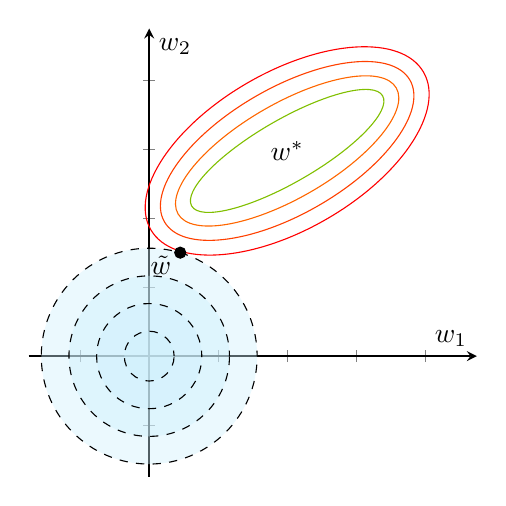
\begin{tikzpicture}

    \begin{axis}
        [
        xticklabels={\empty},
        yticklabels={\empty},
        xlabel={$w_1$},
        ylabel={$w_2$},
        ymajorgrids=false,
        xmajorgrids=false,
        axis line style = semithick,
        ymin=-3.5, ymax=9.5,
        xmin=-3.5, xmax=9.5,
        axis lines=middle,
        axis equal image,
%        xtick=\empty,
%        ytick={4},
        yticklabels={$a$},
        ]
        \def\ex{4};
        \def\ey{5.95};
        \def\rot{-60};

        \plotregularizercontour{3.9em}{}
        \plotregularizercontour{2.9em}{}
        \plotregularizercontour{1.9em}{}
        \plotregularizercontour{0.9em}{}

        % J contour
        \plotobjectivecontour{\ex}{\ey}{1.0cm}{2.0cm}{\rot}{red}
        \plotobjectivecontour{\ex}{\ey}{0.8cm}{1.8cm}{\rot}{red!50!orange}
        \plotobjectivecontour{\ex}{\ey}{0.6cm}{1.6cm}{\rot}{red!20!orange}
        \plotobjectivecontour{\ex}{\ey}{0.4cm}{1.4cm}{\rot}{orange!50!green}
        \node[] at (\ex, \ey) {$\bm{w}^*$}; % <---

        % \tilde{w}
        \addplot[color=black, draw opacity=1, mark=*] coordinates {(0.9,3)};
        \node[anchor=north east, shape=circle, fill=white, fill opacity=0.0, text opacity=1] at (0.9,3.2) {$\tilde{\bm{w}}$}; % <---

    \end{axis}
\end{tikzpicture}